\documentclass[conference]{IEEEtran}
\IEEEoverridecommandlockouts
% The preceding line is only needed to identify funding in the first footnote. If that is unneeded, please comment it out.
\usepackage{cite}
\usepackage{amsmath,amssymb,amsfonts}
\usepackage{algorithmic}
\usepackage{graphicx}
\usepackage{textcomp}
\usepackage{xcolor}
\def\BibTeX{{\rm B\kern-.05em{\sc i\kern-.025em b}\kern-.08em
    T\kern-.1667em\lower.7ex\hbox{E}\kern-.125emX}}
\begin{document}

\title{Day Ahead Load Forecasting for the Modern Distribution Network - A Tasmanian Case Study}

\author{\IEEEauthorblockN{Michael Jurasovic}
\IEEEauthorblockA{\textit{Engineering~~} \\
\textit{UTAS~~}\\
Hobart~ \\
mjj4@utas.edu.au}
\and
\IEEEauthorblockN{Evan Franklin}
\IEEEauthorblockA{\textit{dept. name of organization (of Aff.)} \\
\textit{name of organization (of Aff.)}\\
City, Country \\
email address}
\and
\IEEEauthorblockN{Michael Negnevitsky}
\IEEEauthorblockA{\textit{dept. name of organization (of Aff.)} \\
\textit{name of organization (of Aff.)}\\
City, Country \\
email address}
\and
\IEEEauthorblockN{Paul Scott}
\IEEEauthorblockA{\textit{dept. name of organization (of Aff.)} \\
\textit{name of organization (of Aff.)}\\
City, Country \\
email address}
}

\maketitle

\begin{abstract}
The transformer neural network architecture was applied to short term load forecasting.
\end{abstract}

\begin{IEEEkeywords}
component, formatting, style, styling, insert
\end{IEEEkeywords}

\section{Introduction}
The modern distribution network has changed more over the last ten years than it has in the previous hundred.
In the past, generation and load were largely separate; power was generated exclusively at large stations, and power was consumed by customers after traversing the transmission and distribution networks. 
These days, power is still consumed in the distribution network, but is also generated and manipulated by distributed energy resources (DER). 
\par
DERs are controllable devices in the power network that generate, store, and consume load. 
This includes solar generation (PV), battery storage, and electric vehicles (EV). 
\par
The Tasmanian distribution network is forecast to experience significant increases in these technologies by 2025: \\
\begin{itemize}
	\item 600\% increase in battery storage capacity (from 100MWh to 600MWh) \cite{Jacobs2017}
	\item 170\% increase in PV installation capacity (from 130MW to 220MW) \cite{Jacobs2017}
	\item 39\% of new car sales will be EVs - the highest in the country \cite{AEMO2016}
\end{itemize}

This changing network presents an opportunity to maximize the use of existing assets by delaying the need for network augmentations, while also providing customers with a more reliable supply of power.
For example, batteries could be used to peak-shift, reducing maximum feeder load.
However, to achieve this requires sophisticated methods to optimize the power flow to and from the distributed resources.
\par
One method to achieve this is presented in \cite{Scott2014} and has been implemented on Bruny Island, Tasmania.
The island is a popular holiday destination and during peak periods, such as Easter morning/afternoon peaks, the submarine feeder supplying the island becomes overloaded and has to be supplemented by a diesel generator located on the island.
The aim of the project was to peak shift the load away from the morning/afternoon and avoid the use of the generator.

The method relies on having an accurate forecast of day-ahead load at the feeder level.
Load forecasting methods commonly employed in industry are neither intended to forecast with high accuracy over a time period this short nor at such a low level in the distribution network \cite{CIGRE2016}.
As a result, the optimization of the distributed resources was not as effective as it could be.
\par
To solve this, a neural network-based load forecasting system is proposed.
This system will be applied to Bruny Island, in southern Tasmania, as a case study.
Bruny Island currently has a high penetration of PV and battery technology which is optimized by the Network-aware Coordination (NAC) algorithm \cite{Evan2016}.
Additionally, it is constrained by its feeder during peak holiday periods, necessitating an on-island diesel generator. The load forecasting system will need to be able to perform equally well on holidays, where the load is generally large, and on normal days. 
This makes it a perfect case study to highlight the potential benefits that distributed resources can have in the network.
This project and case study is supported by TasNetworks.


\section{Proposed Forecasting System}
Recurrent Neural Networks (RNN) have recently been popular for load forecasting \cite{Kong2018}.
However, RNNs have been out-performed by the Transformer \cite{Vaswani2017} model in several domains including machine translation \cite{Vaswani2017} (where the architecture was first proposed and applied), medical time series forecasting and regression \cite{Song2017}, and image generation \cite{Parmar2018}.
\par
The proposed forecasting system uses a Transformer neural network model combined with similar load profile selection.
\par
Given a multivariate time series $X = (\boldsymbol{x}_1, ..., \boldsymbol{x}_P)$, with $\boldsymbol{x}_t \in \mathbb{R}^S$ denoting a point in time comprised of $S$ observations (a single point in an S-variate time series), the forecasting system produces a univariate time series forecast $Y = (\boldsymbol{y}_1, ..., \boldsymbol{y}_R)$ with $\boldsymbol{y}_t \in \mathbb{R}^1$.
\par
The points in $X$ and $Y$ are evenly spaced, e.g. 30 or 60 minutes apart, and this is the same for both $X$ and $Y$.
$X$ and $Y$ are aligned on any five minute interval, allowing the forecast to be updated every five minutes.


\subsection{Similar Profile Selection}
A load profile (profile for short) is a time series of electrical load over some period of time.
In this paper, all profiles are measured in kVA and are univariate. 

Load profiles are influenced by exogenous factors such as weather, day of the week, and holiday type \cite{Weron2006}.
Holiday type indicates which holiday the profile occurs on - Easter or Christmas for example.
These different holidays are assigned different integer identifiers (with normal days assigned identifier 0) to form a time series.
The forecasting system was provided with historical load profiles with similar exogenous data to the profile being forecast.
\par
Similar profiles were identified by first finding candidate similar profiles an integer multiple of 1 year $\pm$30 days away from the profile being forecast and filtering the candidates down to profiles with exactly matching hour and minute.
The hour and minute used were in local time to account for changes around daylight savings.

Then the weighted Euclidean distance between the profile being forecast and each candidate profile was calculated using the following features: maximum future temperature, minimum future temperature, day of week at the time of the first point in the forecast, holiday type at the time of the first point in the forecast, and maximum past load.
How far into the future/past the model acquires these values from is dictated by the model parameters.
Typically, a value of 24 hours is chosen for looking into the past, and looking into the future is limited to the forecast horizon.
The candidate profiles with the lowest distance were selected to be used as input, and their corresponding historical weather data was also supplied as an input.
\par
When training and testing the model the similar days were selected from both the past and the future, as the train and test datasets were only five years each.
\subsection{Transformer}
The transformer neural network architecture, shown in figure \ref{fig:transformer}, was introduced by \cite{Vaswani2017} in 2017 and at the time was the state of the art in neural machine translation.
This architecture follows the standard sequence-to-sequence/encoder-decoder architecture: the encoder transforms an input $X = (\boldsymbol{x}_1, ..., \boldsymbol{x}_P)$ into a latent representation $Z = (\boldsymbol{z}_1, ..., \boldsymbol{z}_Q)$, and the decoder transforms $Z$ into an output sequence $Y = (\boldsymbol{y}_1, ..., \boldsymbol{y}_R)$.

The encoder is constructed of a stack of $L$ identical layers, each containing two sub-layers.
The first is multi-head self-attention and the second is a position-wise feed-foward network, both discussed below.
Both sub-layers have a residual connection around them and are fed into a normalization layer.

The decoder is similar to the encoder except for a third layer which implements multi-head attention on the outputs of the encoder - the attention queries come from the previous decoder layer, while the keys and values come from the encoder output.
The input to the decoder is the previous output of the decoder, but shifted right by one and with every value not yet predicted set to zero.
This requires an iterative approach to be used to predict all points in the time series.
The self-attention in the decoder is masked so that when evaluating a query at time $t$ it is unable to assign large weights to keys/values occurring after $t$ in time - ensuring the decoder is autoregressive.

The individual sections of the transformer are discussed in the following sections.

\begin{figure}[htbp]
	\centerline{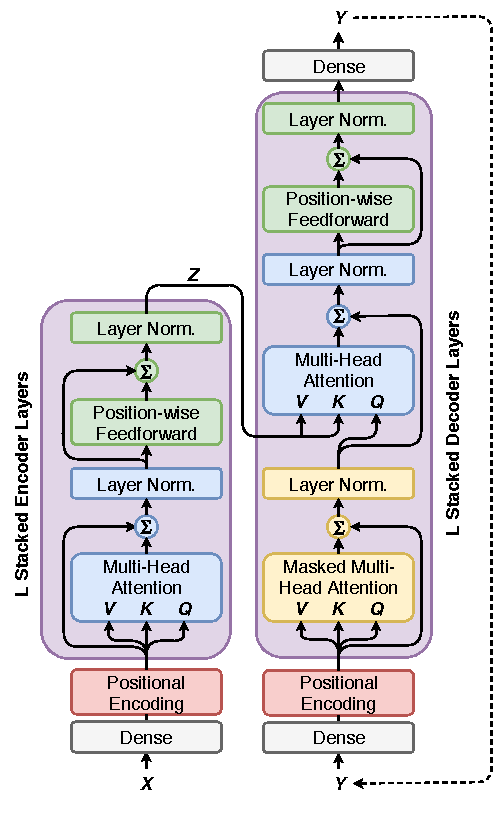
\includegraphics[width=.35\textwidth]{images/transformer.pdf}}
	\caption{The Transformer architecture.}
	\label{fig:transformer}
\end{figure}

\subsection{Input Embedding}
The input $\boldsymbol{X} \in \mathbb{R}^{T \times N}$, where the rows represent $T$ points in time and the columns represent $N$ time series, is embedded by applying a dense layer to produce an embedded $\boldsymbol{Y} \in \mathbb{R}^{T \times d}$, with $d$ being the hidden dimension of of the model.
This is intended to allow the neural network to learn the relationships and dependencies between the different input time series.
The embedded representation is given by Equation \ref{dense_layer}, with learned weights $\boldsymbol{W} \in \mathbb{R}^{N \times d}$ and a learned bias vector $\boldsymbol{b} \in \mathbb{R}^{d}$.

\begin{equation} \label{dense_layer}
\boldsymbol{Y} = \text{max}(0, \boldsymbol{XW} + \boldsymbol{b})
\end{equation}

\subsection{Positional Encoding}
The model has no way of telling the position or order of each element in the input, so this information is injected in the positional encoding layer.
This is done by using a learned lookup table to add the same value to the inputs at both test and train time depending on their position in time in the input.
Specifically, a matrix lookup table of embeddings $\boldsymbol{E} \in \mathbb{R}^{T \times d}$ is added to the embedded inputs as per Equation \ref{positional_encoding}.
\begin{equation}\label{positional_encoding}
\boldsymbol{Y} = \boldsymbol{X} + \boldsymbol{E}
\end{equation}

\subsection{Multi-Head Attention} \label{multihead_attention}
The primary innovation of the Transformer architecture is multi-head attention.
Generic attention and dot-product attention will now be described as these are prerequisite to describing multi-head attention.

Given a single query vector and a set of key and value pairs (with each key and each value being a vector), an attention function matches the query to the keys to produce a weight for each key.
These key weights are then used to create an output vector comprised of the weighted sum of the values, where each value's weight is the weight assigned to its corresponding key. 
Matching of the query to the keys is performed with an arbitrary fitness function.

Scaled dot-product attention, shown in Figure \ref{fig:multihead} (left), is a specific implementation of an attention function. 
It uses the dot product of the query and each key to generate the weights, which are then passed through a softmax function such that the sum of all weights is equal to 1.
In practice, the query row vectors are combined into a single matrix, $\boldsymbol{Q}$, allowing computationally cheap matrix calculations to be used to evaluate the attention outputs in parallel.
The keys and values are represented by row vectors in $\boldsymbol{K}$ and $\boldsymbol{V}$, respectively.

The dot product of the keys and queries is scaled (hence the name) by multiplying it by $\frac{1}{\sqrt{d_k}}$, with $d_k$ being the key and query dimension, to prevent the dot product from becoming large when $d_k$ is large.
A large dot product may cause the gradient of the softmax function to become small and cause issues with training of the model.

The causal mask shown in Figure \ref{fig:multihead} is used exclusively in the decoder self-attention (where $\boldsymbol{Q}$, $\boldsymbol{K}$ and $\boldsymbol{V}$ are identical) to prevent the attention function from matching any query to a key that occurs after itself in time.
This is achieved by leaving the lower triangular portion of the matrix untouched and setting the other values to be large negative numbers - indicating a very poor match.

Multi-head attention, shown in Figure \ref{fig:multihead} (right), applies a separate dense layer to each of the values, queries, and keys. 
The dense layer is applied per Equation \ref{dense_layer} with learned weights $\boldsymbol{W} \in \mathbb{R}^{d \times d}$ and a learned bias vector $\boldsymbol{b} \in \mathbb{R}^{d}$.
The outputs of the dense layers are then split along the last axis into $h$ sets, or heads.
As a result the key, query, and value dimension is reduced by a factor of $h$ to $\frac{d}{h}$.
Scaled dot-product attention is then run independently on each set.
The results are concatenated and put through a final dense layer to produce the output of the attention function.
The dense layer function on the output is defined by Equation \ref{dense_layer} where $\boldsymbol{W} \in \mathbb{R}^{d \times d}$ is a learned weight matrix and $\boldsymbol{b} \in \mathbb{R}^{d}$ is a learned bias vector.

The theory behind multi-head attention is that the dense layer combined with the split allows the model to pick out information from different subspaces in the input and direct these to different attention heads.
This supposedly improves performance over a single head.

\begin{figure}[htbp]
	\centerline{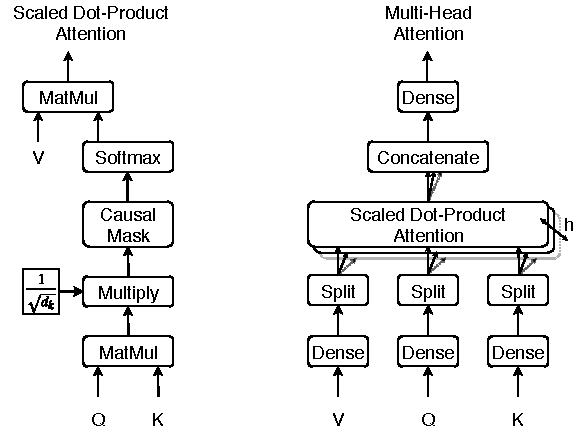
\includegraphics[width=.35\textwidth]{images/multihead_attn.pdf}}
	\caption{Multiheaded attention (right) splits the key, query, and value matrices and applies scaled dot product attention (left) on each in parallel before concatenating the result to return the data to its original dimension.}
	\label{fig:multihead}
\end{figure}

\subsection{Feed-forward}
The feed-forward layer is a two layer network that is applied identically to each time step.
Given an input $\boldsymbol{X} \in \mathbb{R}^{T \times d}$, the output $\boldsymbol{Y} \in \mathbb{R}^{T \times d}$ is populated by Equation \ref{feedforward} where $\boldsymbol{W}_1 \in \mathbb{R}^{d \times 4d}$, $\boldsymbol{b}_1 \in \mathbb{R}^{4d}$, $\boldsymbol{W}_2 \in \mathbb{R}^{4d \times d}$, and $\boldsymbol{b}_2 \in \mathbb{R}^{d}$ are learned weights and biases.

\begin{equation} \label{feedforward}
\boldsymbol{Y} = \text{max}(0, \boldsymbol{X}  \boldsymbol{W}_1 + \boldsymbol{b}_1)  \boldsymbol{W}_2 + \boldsymbol{b}_2
\end{equation}

\subsection{Decoder Dense Output}
The output of the decoder is passed through a dense layer to project the hidden dimension to the desired dimension of 1.
The layer is implemented per Equation \ref{dense_layer} where $\boldsymbol{W} \in \mathbb{R}^{d \times 1}$ is a learned weight matrix and $\boldsymbol{b} \in \mathbb{R}^{1}$ is a learned bias vector.



\subsection{Addition \& Normalization}
Residual connections \cite{He2015} are applied around each sub-layer.
That is, the output of each sub-layer is given by $\boldsymbol{Y} = \boldsymbol{X} + \text{subLayer}(\boldsymbol{X})$ where subLayer$(\boldsymbol{X})$ is the original output of the sub-layer.
The outputs are then normalized by applying layer normalization \cite{Ba2016}, as per Equation \ref{layernorm} where $\mu_{\boldsymbol{x}}$ and $\sigma_{\boldsymbol{x}}$ are the mean and variance of $\boldsymbol{x}$ respectively.

\begin{equation} \label{layernorm}
\boldsymbol{Y}_{i,*} = \frac{\mu_{\boldsymbol{X}_{i,*}}}{\sigma_{\boldsymbol{X}_{i,*}}}
\end{equation}

\subsection{Dropout and Training}
Dropout is applied in the following positions:
\begin{itemize}
	\item At the output of the positional encoding of both the encoder and decoder.
	\item Immediately after the softmax operation in the scaled dot-product attention.
\end{itemize}
The model is trained using the Adam optimizer \cite{Kingma2014}.
The loss function is a modified sum squared error.
Given a vector $\boldsymbol{y}$ of predictions from the model and a vector $\boldsymbol{y'}$ of expected predictions the loss function $l$ is given by 
\begin{equation}
l = \sum_{t=0}^{U}((\boldsymbol{y}_t^2 - \boldsymbol{y'}_t^2) \times |\boldsymbol{y'}_t|^c)
\end{equation}
Where $c$ is a model hyperparameter.
For $c>0$ this function accentuates loss when the actual value is large - this is useful for a load forecast as times of maximum demand are likely important for planning purposes.
When $c=0$ this is simply normal sum squared error, and for $c<0$ this will accentuate loss when the actual value is small.

When testing or being used for inference, the decoder outputs are generated sequentially one at a time.
Values that have not yet been generated are set to zero.
These zero values do not affect the output of the decoder, as the decoder self-attention is masked so that it does not make use of them.
After each output value is generated, it is populated in the decoder input.
When training, the decoder input is set to the known expected value and the model is executed a single time.


\section{Case Study}
The forecasting system was applied to Bruny Island.

\subsection{Bruny Island}
(Discuss briefly the location of Bruny Island - Figure \ref{fig:bruny_map}) and Figure \ref{fig:bruny_network}.
(Discuss briefly the NAC and batteries).
Discuss requirements of forecasting system for Bruny.
Discuss typical patterns on Bruny - a graph or two.

Bruny Island, shown in Figure \ref{fig:bruny_map}, is located approximately 2 kilometres off the coast of south-east Tasmania with a permanent resident population of approximately 800 people \cite{census2016}.
The island is a popular holiday destination, with Easter periods typically experiencing an influx of up to 500 cars in a single day. \textbf{(Citation? This comes from council data)}


\begin{figure}[htbp]
	\centerline{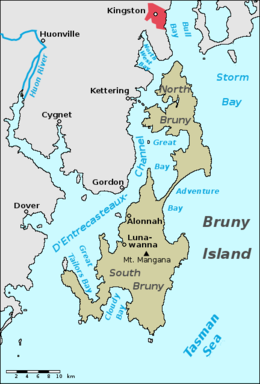
\includegraphics[width=.35\textwidth]{images/bruny_island_map.png}}
	\caption{Placeholder showing location of Bruny Island relative to Australia/Tasmania. From Wikipedia - todo reproduce.}
	\label{fig:bruny_map}
\end{figure}

\begin{figure}[htbp]
	\centerline{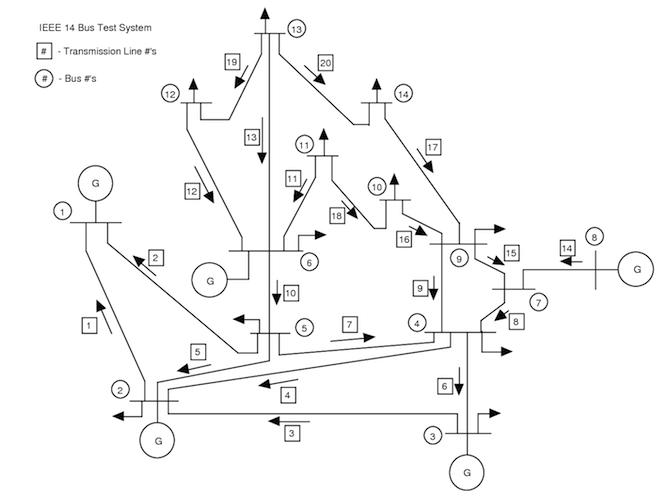
\includegraphics[width=.35\textwidth]{images/bruny_network.png}}
	\caption{Placeholder showing layout of distribution network on Bruny. Shows locations of reclosers and feeders - todo reproduce.}
	\label{fig:bruny_network}
\end{figure}

\subsection{Data}
Discussion of available data and what was supplied to the forecasting system.
The following data was available for Bruny Island
\begin{itemize}
	\item One-minute resolution total apparent power consumption for Bruny Island, and downstream reclosers from 2009-2018
	\item One-minute resolution temperature, humidity, wind, and solar data from a site located 50km from the island from 2009-2018. 
	\item One-minute resolution total apparent power consumption at  St Helens. 
\end{itemize}

\subsection{Forecasting Model Configuration}
The forecasting system was configured with the parameters in table ... .
[Horizon: 24 hours, period: 30 minutes, 5 similar days, ]


\subsection{Results}
Results of case study.

Present evaluation based on historical data, focussing on holiday periods.

Present briefly the event where the generator did not have to start.

\section{Conclusion}
Blah Blah the forecaster works.
Used a Transformer model.
Applied to Bruny Island and NAC, helped prevent generator from turning on.
Maybe something about future work?


\section*{Acknowledgment}
TNW


\bibliographystyle{IEEEtran}
\bibliography{aupec}

\section{Notes questions etc.} 
\begin{itemize}
	\item Are references formatted properly? And do they include sufficient information like journal etc.? \\
	TODO fill in more journal info.
	\item Matrix subscript notation $\boldsymbol{X}_i,j$ for single element, $\boldsymbol{X}_i,*$ for single row, and $\boldsymbol{X}_*,j$ for single column. Could leave like this, could add a footnote, could change. \\
	$\boldsymbol{X}_i,*$ This appears to be fairly common notation, or at least one of several more commonly used notations.
	\item Maybe use $\boldsymbol{X} \in \mathbb{R}^{N \times T}$ rather than $\boldsymbol{X}$ is a matrix of dimension $N \times T$? \\
	Yep, done.
	\item ummm not enough equations? I have specified the model in a way that is intended to be easy to follow and implement which tends toward specifying multiplications etc using words rather than abstract equations.\\
	Put the inline equations into their own lines.
	\item When reading the sections describing the transformer please also compare this to the paper Attention Is All You Need. This was the paper that originally published the Transformer and I am a little concerned that my descriptions, which are certainly inspired by the original paper, are a little too similar.
	\item Notation of matrices $\boldsymbol{X}$ (bold capital), vectors $\boldsymbol{x}$ (bold lowercase), and scalars $x$ (lowercase). Appropriate? \\
	yea looks good.
	\item When specifying $\boldsymbol{X}_i,j = ...$ should I say for $i= 1..n, j= 1..m$? \\
	unnecessary probably.
\end{itemize}

\end{document}
